\part{Problème de satisfaction de contraintes CSP}
\pagebreak

\chapter{Introduction et modèles}
\pagebreak

Une Solution d'un problème CSP est une assignation d'une valeur à chaque variables de P tel que toutes les contraintes de P soit satisfaite.\\

\section{exemple simple}

Trouver une assignation Minimal et Maximal pour chaque variables de P dans le problème suivant:\\
\begin{description}
\item[vars(P)] = $w,x,y,z$
\item[Dom(P)]\  \begin{description}
\item[Dom(w,x)] = $\{1,2,3\}$
\item[Dom(y,z)] = $range(4)$
\end{description}
\item[Contraintes]\  \begin{description}
\item[$~$] $w = x$
\item[$~$] $x \leq y + 1$
\item[$~$] $y > z$
\item[$~$] $(x,z) \in \{(1,2),(2,1),(2,4),(3,3)\}$
\end{description}
\end{description}
\ \\
Une solution serait:
\begin{description}
\item[Minimal] $w=x=1, y=3, z=2$
\item[Maximal] $w=x=z=3, y=4$
\end{description}

\pagebreak
\subsection{Graphe de contraintes}

Chaque variable est un nœud et chaque contraintes est représenté par une arête entre les variables concerné.\\
\begin{center}
\begin{tikzpicture}[-,>=stealth',shorten >=1pt,auto,node distance=2.8cm,
                    semithick]
  \tikzstyle{every state}=[fill=white,draw=none,text=black]

  \node[state]         (W)                    {$W$};
  \node[state]         (X) [left of=W]        {$X$};
  \node[state]         (Y) [below right of=X] {$Y$};
  \node[state]		   (Z) [below left of=X]  {$Z$};
  

  \path (X) edge              node {} (W)
            edge              node {} (Y)
            edge			  node {} (Z)
        (Z) edge			  node {} (Y);
\end{tikzpicture}
\end{center}
\subsection{Graphe de compatibilité}

Représenter toutes variables avec des ensemble contenant toutes les valeur de leurs domaine puis relier chaque éléments de l'ensemble avec un autre tel que les contraintes ne soit pas violet:\\
\begin{center}
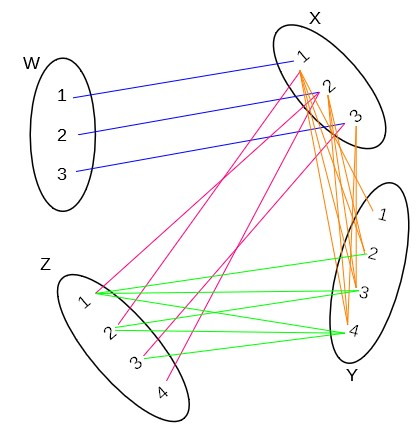
\includegraphics[scale=0.6]{img/aic_csp_1.jpg} 
\end{center}
\pagebreak

